\icode[magenta]{E-ME-MU-L4-261019-001}
（多选）
如图所示，一质量为\qty{1}{\kg}的小球穿在一足够长、粗糙的细杆上，杆与水平方向夹角\(\theta =\) \,\qty{37}{\degree}，小球与细杆间的动摩擦因数\(\mu = 0.5\)。将小球从A点静止释放的同时加上一垂直于杆向上的外力\(F\)，\(F\)的大小随时间变化的规律为\(F = 4t\) (\qty{}{SI})，经过一段时间后，小球停止运动。重力加速度\(g =\) \,\qty{10}{m/s^2}，\(\cos\) \,\qty{37}{\degree}=0.8，\(\sin\)\,\qty{37}{\degree}=0.6，对小球运动的全过程，下列说法正确的是\paren[]

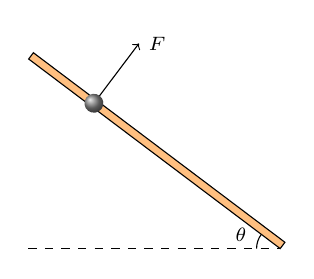
\begin{tikzpicture}[font=\scriptsize]
	\begin{scope}[rotate=-37]
	\draw[fill=orange!50] (0,0) rectangle(-4,0.1);
	\draw[->] (-3,0)--(-3,1)node[right]{\(F\)};
	\shade[ball color=gray] (-3,0.05) circle(.12);
	\end{scope}
	\draw[dashed] (-3.2,0)--(0,0);
	\draw (-.3,0) arc(180:143:.3);
	\node at(-.5,.18) {\(\theta\)};
\end{tikzpicture}
\begin{choices}
	\item 小球与细杆间最大摩擦力为\qty{4}{N}
	\item 小球重力势能减少量等于摩擦生热量
	\item 小球的最大动量为\qty{17}{kg\cdot m/s}
	\item 小球的最大加速度为\qty{6}{m/s^2}
\end{choices}
\begin{answer}
	BD\qquad 提示：
\end{answer}